%% LyX 2.2.1 created this file.  For more info, see http://www.lyx.org/.
%% Do not edit unless you really know what you are doing.
\documentclass[sigconf,anonymous=false,authordraft=false]{acmart}
\usepackage[latin9]{inputenc}
\usepackage{verbatim}
\usepackage{float}
\usepackage{url}
\usepackage{enumitem}
\usepackage{graphicx}

\makeatletter
%%%%%%%%%%%%%%%%%%%%%%%%%%%%%% Textclass specific LaTeX commands.
\newlength{\lyxlabelwidth}      % auxiliary length 

%%%%%%%%%%%%%%%%%%%%%%%%%%%%%% User specified LaTeX commands.
%\renewcommand\footnotetextcopyrightpermission[1]{} % removes footnote with conference information in first column
%\pagestyle{plain} % removes running headers


%\makeatletter
%\renewcommand\@formatdoi[1]{\ignorespaces}
%\makeatother


\usepackage{url}
\usepackage{enumitem}
\usepackage{amstext}
\usepackage{graphicx}
\usepackage{booktabs} % For formal tables



\usepackage{subfigure}
\usepackage[ruled,vlined,linesnumbered]{algorithm2e}

\newcommand\varlist{,\makebox[0.8em][c]{.\hfil.\hfil.},} 

% DOI
\acmDOI{10.475/123_4}

% ISBN
\acmISBN{123-4567-24-567/08/06}

%Conference
\acmConference[WOODSTOCK'97]{ACM Woodstock conference}{July 1997}{El
  Paso, Texas USA} 
\acmYear{1997}
\copyrightyear{2016}

\acmPrice{15.00}

\fancyhead{}
\settopmatter{printacmref=false, printfolios=false}

\newcommand{\I}{\mathbb{I}}
\newcommand{\N}{\mathcal{N}}
\newcommand{\E}{\mathrm{E}}
\newcommand{\Ind}{\mathrm{\#}}
\renewcommand{\vec}[1]{\mathbf{#1}}
\newcommand{\Sim}{\mathrm{Sim}}
\newcommand{\ExpOneCall}{\text{Exp-}1\text{-Call@}k}
\newcommand{\PLAR}{\text{PLAR}}

\newcommand{\heq}{\hspace{-.5mm} = \hspace{-.5mm}}
\newcommand{\seq}{\hspace{-1mm} = \hspace{-1mm}}



\newcommand{\ExpNCall}[1]{\text{Exp-}#1\text{-Call@}k}
\newcommand{\TlessK}{T_{\!\!\:k\text{-}1}}
\def\argmax{\operatornamewithlimits{\!arg \;\! max\,}}

\makeatother

\begin{document}
%\title{VTF: A Filter Selection-Based Search Tool for Social Network Visualization} 
%\title{VTF: A Visual Filter Selection-Based Search Tool for Social Network} 
%\title{Viz-TSF: A Visual Twitter Search Tool based on the Filtering of Geo-Temporally Coherent Content}
\title{Viz-TSF: A Visual Twitter Search Tool based on Query-driven Filter Optimization}
\author{Mohamed Reda Bouadjenek}
%\orcid{1234-5678-9012}
\affiliation{%
  \institution{The University of Toronto}
  \streetaddress{Department of Mechanical and\\ Industrial Engineering}
  \city{Toronto} 
  \state{Ontario} 
   \postcode{M5S 3G8}
  \country{Canada}
}
\email{mrb@mie.utoronto.ca}

\author{Scott Sanner}
\affiliation{%
  \institution{The University of Toronto}
  \streetaddress{Department of Mechanical and\\ Industrial Engineering}
  \city{Toronto} 
  \state{Ontario} 
   \postcode{M5S 3G8}
  \country{Canada}
}
\email{ssanner@mie.utoronto.ca }



\newcommand{\subfour}[1]{\vspace*{3mm}{\noindent\bf #1}}  
\newcommand{\subsubfour}[1]{\vspace*{1mm}{\noindent\bf #1}} 
\begin{abstract}
Geo-temporal visualization of Twitter search results is a challenging task since the simultaneous display of all matching tweets would result in a saturated and unreadable display. Thus, the development of novel intuitive visual interfaces is necessary to help focus a user's attention by filtering information relevant to their query. In this work, we propose a Visual Tweet Search Filter (Viz-TSF) tool for query-driven optimization and ranking of spatial, temporal, and content-based filters to help focus a user's exploration of search results.  We leverage a fast greedy optimization algorithm to optimize an approximation of expected F1-Score metric to generate these filters and demonstrate its application to search 2 years of Twitter content, specifically for a user's information need related to natural disasters occurring in the US.  Our demo shows that Viz-TSF is capable of extracting geo-temporally coherent filters given search queries, thus aiding the user in visually searching and browsing social network content and enabling new opportunities for the application of Information Retrieval techniques to general visual information exploration interfaces.

\noindent {\bf Keywords:} Adaptive UIs; Visual Search Interfaces;
Optimization for IR.
\end{abstract}
\maketitle

\section{Introduction}

Traditional search engines such as Google or Bing display search results
in a vertical list of textual summaries. However, this display mode
is certainly not adapted for search results over Twitter content,
since related tweets are often geographically and temporally localized. Moreover, given
the massive volume of available information in Twitter, displaying
all relevant tweets for a given query prevents the visual extraction
of relevant information as it would result in a saturated and unreadable
display \cite{Liu2014}. Thus, adaptive user interfaces (AUIs) are
necessary to filter information to provide localized and relevant
tweets for each query. Such AUIs would allow the user to efficiently explore
the content of the matching tweets and to identify key properties
(author, timestamp, geolocation) relevant to the fulfillment of the user's information need.
To this end, we propose a Visual Tweet Search Filter (Viz-TSF)\footnote{\url{http://130.220.208.198:8080/AUI4IRSearch/}}
tool to optimize and rank spatial, temporal, and content-based
filters intended to focus a user's exploration of Twitter search results.  

%The key difference is that while information retrieval is ubiquitous in the lives of most humans in the form of web search, it has gone virtually unrecognize as an appropriate model for the filtering problem in AUIs \textcolor{red}{[REFERENCE IS NEEDED]}. 
%Instead, machine learning methods have been widely used to address this problem.

\begin{figure}[t]
% \subfigure[Global display showing anomalies.]{\includegraphics[width=4.25cm]{imgs/twitter_example}\label{Fig:GlobalDisplay}}\subfigure[Filtered and focused display.]{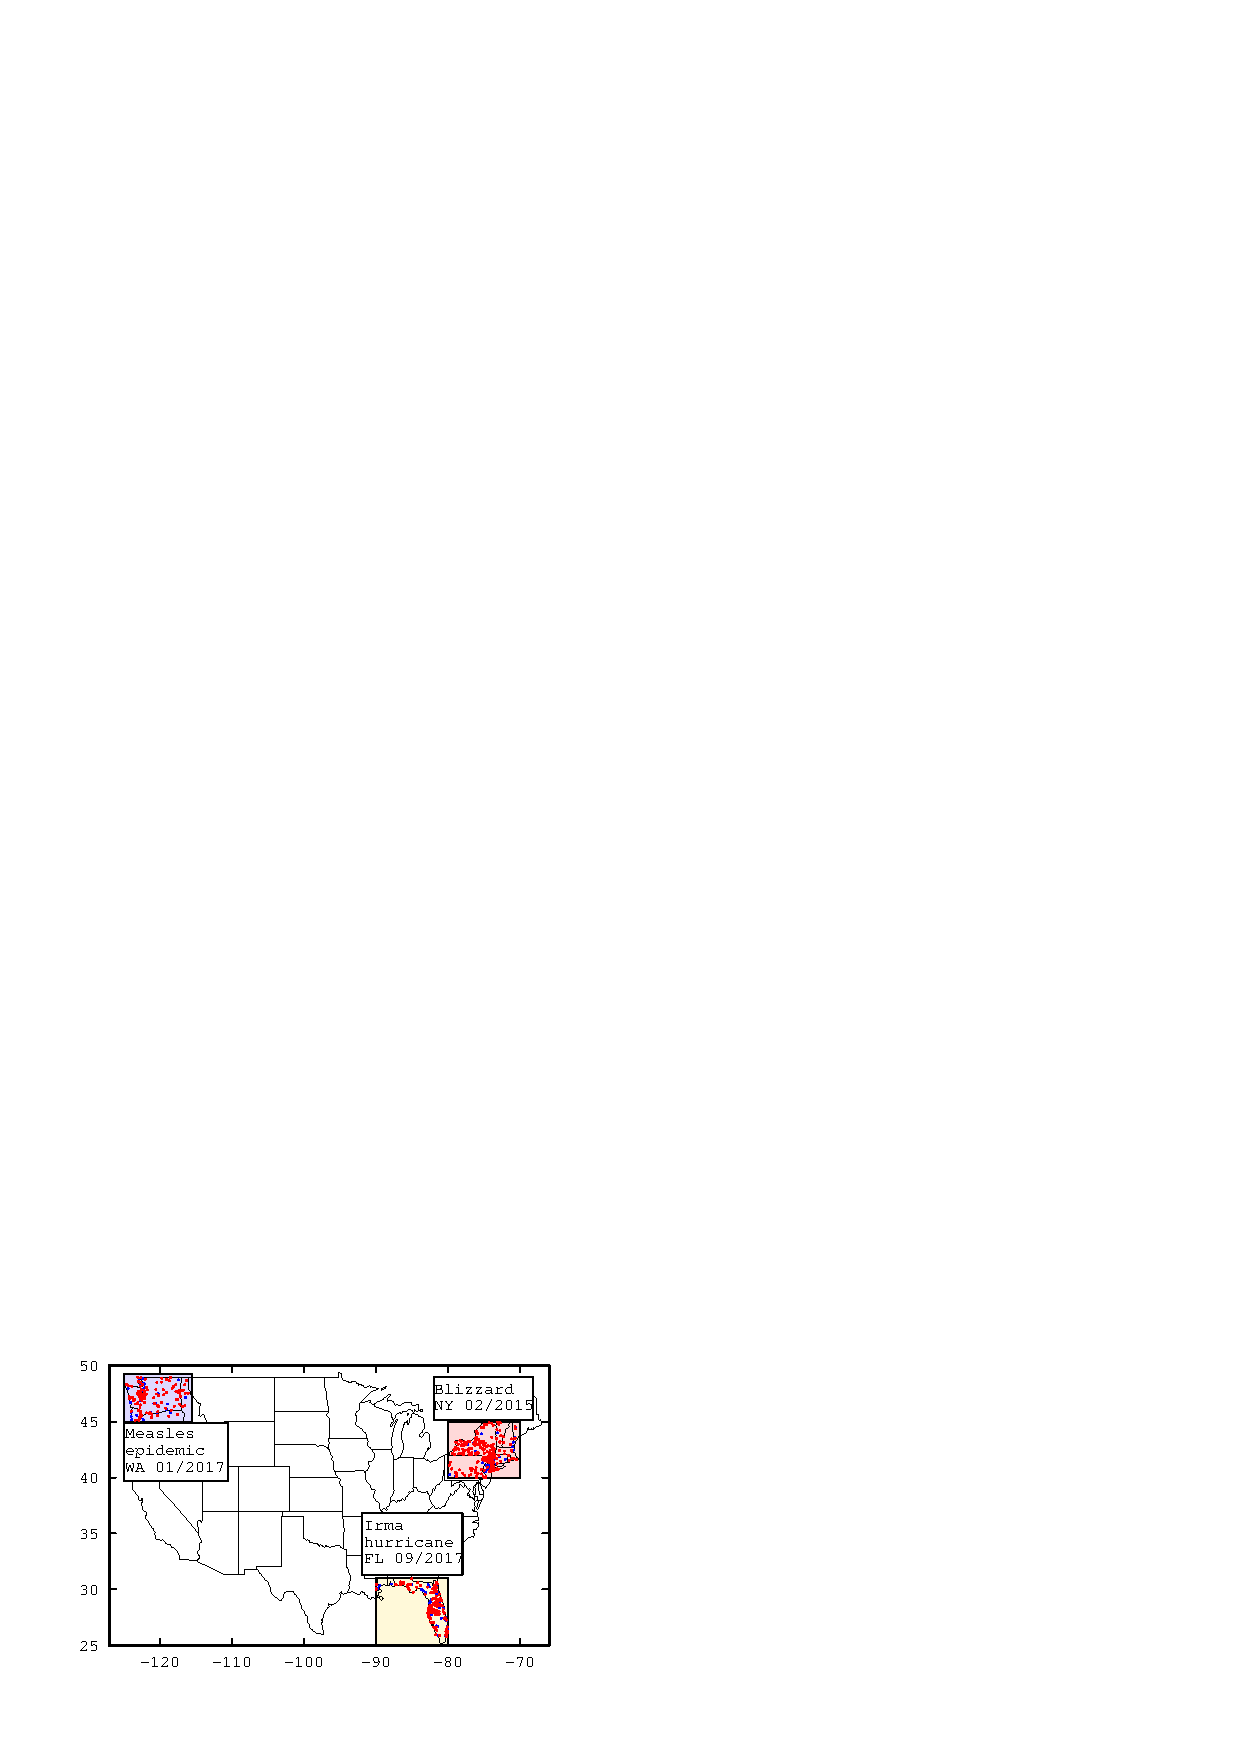
\includegraphics[width=4.25cm]{imgs/twitter_example_filter}\label{Fig:FilteredDisplay}}

\begin{centering}
\subfigure[Global display showing search results.]{\includegraphics[width=7cm]{imgs/map}\label{Fig:GlobalDisplay}}
\par\end{centering}
\begin{centering}
\subfigure[Filtered and focused search interface.]{\includegraphics[width=7cm]{imgs/filtered_map}\label{Fig:FilteredDisplay}} 
\par\end{centering}
\caption{(a) An unfiltered user search interface with geolocated tweets that
best match a query related to natural disaster highlighted in red. (b) A filter-optimized version
of the interface showing the top three filtered subsets of data identified
to have high coverage of relevant content related to the query: a
bounding box near New York state limited to data in Feb 2015 and having
keyword ``Blizzard'' and other time and keyword restricted bounding
boxes centered on Florida and Washington state. }
\label{Fig:UseCase} 
\end{figure}

% \begin{table*}[t]
% \caption{Comparison between conventional Web Search and Filtering for AUIs.}
% \label{tbl:Comparaison2IR}
% \centering{}%
% \begin{tabular}{|c|>{\centering}p{6cm}|>{\centering}p{6cm}|}
% \hline 
%  & \textbf{Web Search} & \textbf{Filtering for AUIs}\tabularnewline
% \hline 
% \hline 
% \textbf{Information Need} & Realized by query  & Selection of an event or alert\tabularnewline
% \hline 
% \textbf{Form of Results} & Ranked list of documents & Filter settings (bounding box in visual display, time ranges, property
% filters) that select a subset of information elements to display\tabularnewline
% \hline 
% \textbf{Relevance Scoring} & Comparison of query and document content (and other relevant information)
% to generate a relevance score, e.g., via TF-IDF or BM25 & Third party application-specific tool (e.g., a machine learning approach)
% that predicts the probability that each information element is relevant
% to the selected alert\tabularnewline
% \hline 
% \textbf{Test Data for Benchmarking} & A set of queries; human-labeled judgments of document relevance to
% each query for a test corpus (i.e., ground truth relevance) & A set of alerts or events; human-labeled judgments of information element relevance
% to a selected alert (i.e., ground truth relevance)\tabularnewline
% \hline 
% \textbf{Evaluation} & Ranking metrics (P@k, AP, etc.) over documents given ground truth
% relevance  & Boolean metrics (e.g., F1-score) and Ranking metrics (P@k, AP, etc.)
% over information elements selected by the filter given ground truth
% relevance \tabularnewline
% \hline 
% \end{tabular}
% \end{table*}

To make the task of AUI filtering
more concrete, we introduce an example search filtering use case
for AUIs. Consider the case of searching events related to natural
disasters that are discussed on Twitter. Typically, as shown in Figure
\ref{Fig:GlobalDisplay}, there would be some visual display of all
tweets that match the query along with highly relevant Tweets shown as red nodes.  %
%in Figure \ref{Fig:GlobalDisplay}. 
%(such as user IP address, Tweet content, Tweet time, geographical coordinates, recent activity details) 
%We denote all displayed tweets
%as an information tweet that could be optionally shown or not.
% Above -- huh?
Displaying
all tweets simultaneously would result in a saturated and an unreadable
display for many queries that return a high volume of matching content. 
To ease the investigation
and search task, users could restrict the tweets displayed through
a variety of filter settings to get a clear overview of individual
events as shown in Figure \ref{Fig:FilteredDisplay} \textendash{}
by panning and zooming in the graph display, by restricting upper
and lower bounds on a time filter, and/or by selecting properties
(e.g., in a drop-down selection or fielded keyword search in fields
such as Tweet content, author, or hashtags).
%\textcolor{red}{Such filter settings are expected to help a monitoring agent to efficiently investigate the cause and implications of the triggered alarm, to identify common properties of the elements involved in that alert, and to initiate appropriate corrective actions in a timely manner.}

While the user would typically find it hard to manually set these
filters to optimally reveal information about specific relevant events
related to his/her query, an AUI that is aware of a probability
estimate that each tweet is relevant to the query could automatically optimize and suggest a ranking of 
filter settings to visually display relevant tweet content with the
least amount of irrelevant clutter.  The user could then more efficiently browse through the subset of tweets provided by 
the ranked filter settings to carry out investigation w.r.t.\ the original information need while covering a large fraction of the relevant content.
%search and investigation by identifying
%common properties of the tweets related to the query that are in the
%same cluster.

\begin{comment}
We assume the prediction of information element relevance to an alert
to be provided by a third-party since this prediction is highly specific
to each particular application setting and not the focus of this work
(see Related Work in Section 6 for further discussion).
\end{comment}

%In this work, we intend to
%focus on the broader problem of AUI filtering in a range of visual
%display applications assuming this relevance predictor is given. However,
%in addition to scoring information elements of direct causal interest
%to the alert, it is likely that the AUI will also contain other related material requiring
%the concurrent display of information.  For example, such a material could be messages exchanged, the time at which these messages were exchanged, etc.
%For example, such a rule could
%be \textquotedblleft if a connection is shown, the IP addresses of
%the two connected machines must also be shown\textquotedblright ,
%which would trigger additional (soft) constraints for the filter optimization.

Since ``retrieved\textquotedblright{} tweets are not individually
selected, but rather chosen through a filter setting (that the user
can further modify), the problem is clearly an optimization problem
of how to restrict filter settings to show the user the most relevant
tweets to his/her query. While this diverges from the standard information
retrieval setting where ranked documents are chosen individually \cite{Baeza-Yates2010},
these additional constraints do not change the overall information
retrieval objective to select relevant information given the user's
information need and constraints of the user interface. %Furthermore, standard information retrieval evaluation benchmarking
%methodology (e.g., the Cranfield paradigm) and metrics such as precision@k
%or average precision are also relevant here (assuming that visual
%saliency can serve as a surrogate method for achieving a visual rank
%ordering of selected information elements).  Unlike information retrieval
%where Boolean metrics such as F-Score are not often used since ranked
%lists are usually limited to the top-10, graphical displays can present
%substantially more information of varying sizes that make precision-recall
%trade-off metrics like F-Score also relevant for evaluation.\textcolor{red}{ [THIS SENCTENCE IS UNCLEAR]}

%With the aim of assisting network monitoring agents in carrying out their daily tasks, we present in this paper a new visual search paradigm for AUIs. 
%% VISUAL SEARCH RESULTS -- VISUAL SEARCH FILTER
%% VISUAL PRESENTATION OF SEARCH RESULTS -- Reda says terminology may be confused

To the best of our knowledge, Viz-TSF is the first tool to address
a visual information retrieval problem for social media as the explicit optimization of spatial, temporal, and content-based filter selection and ranking w.r.t.\ surrogates of F1-Score well-suited to this task.

% The contributions of this paper are summarized as follows: 
%  \begin{enumerate}
% \item We propose a new theory of IR for adaptive visual user interfaces. 
% \item We propose new expected metrics for optimization based on conventional IR metrics, i.e., precision, recall, and F1-Score.
% We argue that F1-Score and hence expected F1-Score is a good metric for this domain.
% \item We propose new filter setting search algorithms based on greedy strategies and optimal solutions. These algorithms are based on the optimization of new proposed metrics.
% %\item  We propose new MILP-based search method, which can also used about justification of new search algorithm.
% \item We present a thorough evaluation on three different datasets to show that the greedy algorithms we propose are a good approximation of the optimal method, and perform well in the presence of noise (i.e., corruption of the ground truth labels).
% %can even perform better with a noisy classifier \textendash{} up to 42\% improvement for a classifier with an accuracy of 60\%. On the other hand, 
% We experimentally demonstrate that the expected F1-Score metric is a good surrogate of F1-Score.
% %specifically with a highly accurate classifier \textendash{} for a classifier with 90\% accuracy, the RMSE is roughly 0.0111).
% \end{enumerate}

\section{V\lowercase{iz}-TSF architecture and features}

The main components of the architecture of Viz-TSF are: 
\begin{enumerate}
\item \emph{Crawler and Indexer.} To find and organize tweets for further
retrieval.
\item \emph{Query Analyzer}. To understand the user's information need.
\item \emph{Scoring Function}. To score the tweets based on their relevance probability w.r.t.\ the query.
\item \emph{Filter Optimization}. To optimize and rank filter settings w.r.t. the scoring function and filtering objective.
\item \emph{Visual Adaptive User Interface}. To present the information to the user in an accessible and interactive form using filters.
\end{enumerate}
While the two first components are common to many IR systems, we briefly
describe in the following the remaining components which are at the
heart of Viz-TSF.

\subsection{Scoring Function}

The filter optimization component of Viz-TSF relies on the optimization
of an approximation of \emph{expected} F1-Score metric. This expectation 
%is computed based on the conditional probability $p(R|t,q)$, i.e.,
is critically based on an estimated conditional probability $p(q|t)$ 
%the probability 
that a tweet $t$ is relevant to the query $q$.  To obtain this probability estimate,
the ranking function component of Viz-TSF uses a language model scoring approach, which assumes that the terms of a query $q$ are ``generated'' by a
probabilistic model based on the content of tweet $t$, thus directly estimating
$p(q|t)$.
%. Hence, given a query
%$q$ and a document $d$, the language model estimates 
%the conditional likelihood $p(a|d)$, i.e., the posterior probability that $d$ generates the
%observed $q$.  
Specifically for this demonstration, we use a Bayesian smoothing
language model using Dirichlet priors as defined in Zhai and Lafferty~\cite{Zhai2001}.

\subsection{Filter Optimization}

The filter optimization component of Viz-TSF relies on the configuration of three sub-filters
to select a subset of relevant tweets for the data visualization interface -- specifically (i) a keyword content sub-filter, (ii) a temporal sub-filter, and (iii) a spatial (location) sub-filter.
A global filter that is generated by \emph{conjoining} these three
sub-filters is used to select the overall subset of relevant tweets for a filter. Each
sub-filter is constructed following a greedy top-down approach while
seeking to optimize an approximation of the expected F1-Score metric.
For efficiency, the algorithm implemented in this module uses a greedy binary
partitioning search, where the algorithm operates by halving the search space of one sub-filter in each iteration. Details
of this algorithm are further provided in~\cite{Bouadjenek2018b}.

In practice, a single conjoint filter setting chosen by the previous algorithm will
narrow the user on a single ``event''.  However, there are likely multiple
events and so the user should have a ranked choice of multiple filters to choose from.  Hence,
after the first filter is produced, all selected tweets by the filter
have their probability scores zeroed out (since they are already covered by one filter). The filtering algorithm is then run
again, where it will inherently focus on a different content set.
This procedure is repeated until the desired number of filters is
reached. The user should then be able to choose among a ranking of  the filters produced as provided in our demonstration interface. 

\begin{comment}
\subfour{Keywords greedy algorithm:} The idea behind the keywords-based
greedy top-down algorithm is the following: given a set of tweets
and an evaluation measure, the algorithm aims to select a set of keywords
to form a negation query in order to exclude a subset of elements
containing these keywords for the purpose of maximizing the evaluation
measure.

Formally, given a keyword query representation $Q_{k}$, the algorithm
aims to select an optimal subset of $k$ terms$T_{k}^{*}\subset E$
(where $|T_{k}^{*}|=k$ and $E$ is the initial set of elements) to
build a negation keyword query $Q_{k}$, i.e. $Q_{k}=\{\neg t_{1}^{*},\dots\neg t_{k}^{*}\}$,
in order to optimize a given evaluation measure, e.g. expected precision,
expected recall, expected F1-Score. This is achieved by building $T_{k}^{*}$
in a greedy manner by choosing the next optimal term $t_{k}^{*}$
given the previous set of optimal term selections $T_{k-1}^{*}=\{t_{1}^{*},\ldots,t_{k-1}^{*}\}$
(assuming $T_{0}^{*}=\emptyset$) using the following selection criterion: 

\begin{equation}
t_{k}^{*}=\argmax_{t_{k}\notin T_{k-1}^{*}}\hspace{-0.3mm}[EF1(E^{*}\textrm{ that satisfies }Q_{k}=\{\neg t_{1}^{*},\dots\neg t_{k}^{*}\})]
\end{equation}

\noindent assuming we use expected F1-Score to assess $E^{*}$, which
is a subset of the initial element set $E$ that satisfy the negation
keyword query $Q_{k}$. In order to reduce the keyword search space,
we propose to use the top 100 terms ranked using mutual information.
\end{comment}


\subsection{Visual Adaptive User Interface}

As shown in Figure~\ref{fig:MainInterface}, we designed an interactive visual interface providing a multi-perspective view consisting of: (i) an interactive map, which presents search results for each filter setting that permits further user-driven adaption of the filters (e.g., spatial refinement through panning and zooming) and pop-up information summaries by clicking on filters or tweets, (ii) a query panel allowing the user to specify a query, refine the time window filter, and tune two search parameters (the number of filters produced and the value
of $\beta$ for the F$_{\beta}$-Measure that is optimized), and (iii) a ranked list of the filters produced with respect to a given query, which can be used to select and (un)hide some filters for more clarity.

\begin{figure*}[t]
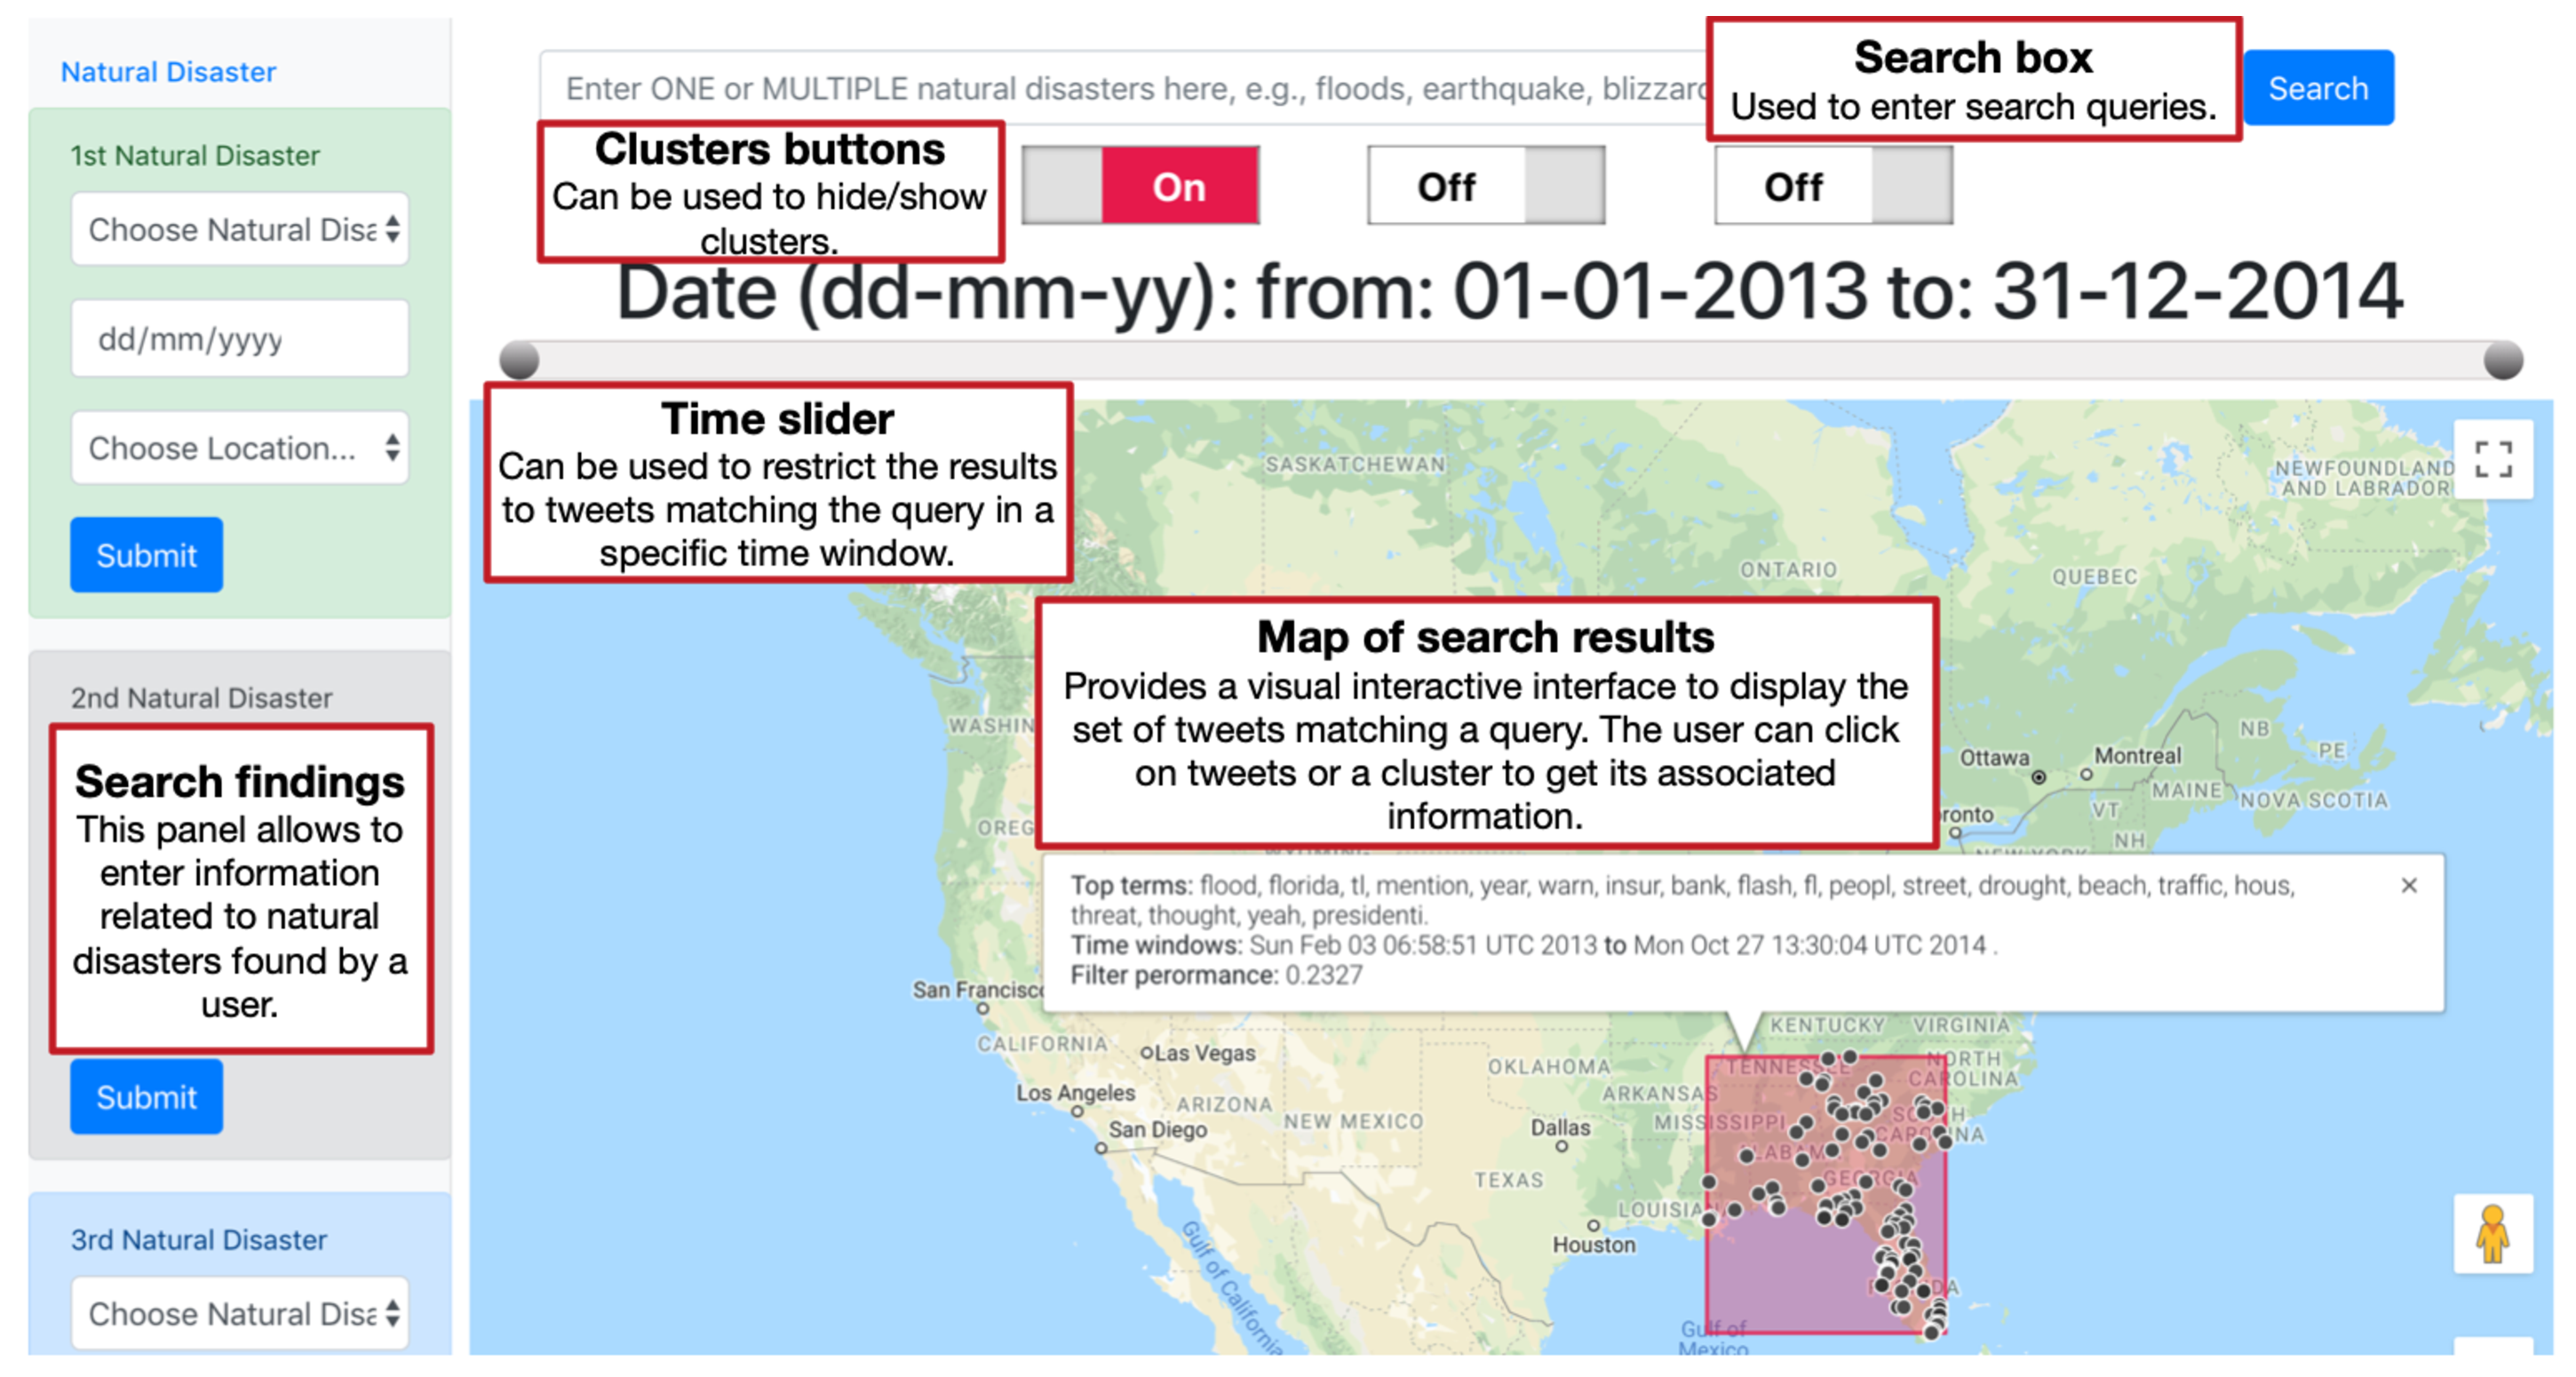
\includegraphics[width=18cm]{imgs/main}

\caption{Main interface of Viz-TSF.}
\label{fig:MainInterface}
\end{figure*}

Viz-TSF is built on the top of the Lucene IR system\footnote{\url{https://lucene.apache.org/core/}}
\cite{McCandless2010} for the indexing, query processing and retrieval
part, and on the Google Maps API for data visualization.

\section{What will be demonstrated?}

This demonstration will be illustrated using Twitter data crawled
using the Twitter Streaming API for two years spanning 2013 and 2014
\cite{Iman2017}. This dataset contains more than 2.5 TB of compressed
data, with a total of 829,026,458 English tweets.

In our demonstration, a user can perform interactive searches such as the following example search scenario:
\begin{itemize}
\item A user begins by searching for information on weather-related natural
disaster events. Using
the querying panel, the user enters a set of keywords ``flood, hurricane, typhoon, drought, storm'', selects a search time window (e.g., January 2013 to June 2014), 
selects the number of filters to be returned, and sets an initial value for
$\beta$. A low value of $\beta$ constrains the algorithm to focus
on the optimization of the precision, thus obtaining filters
with small clusters, whereas a high value of $\beta$ leads to high recall filter settings with large clusters.
%constrains the
%algorithm to focus on the optimization of the recall, thus obtaining
%filters with large clusters. 
The value of $\beta$ can be interactive and iteratively tuned by the user until the desired granularity or coarseness of filter results are obtained.
\item As shown in Figure \ref{fig:main2}, a list of filters is suggested
to the user and displayed on the main map (in this case restricted to the US) along with relevant tweets for the search query, where 
red nodes indicate highly relevant tweets, and blue nodes indicate lower relevance tweets.
\end{itemize}
\begin{figure}[H]
\begin{centering}
\includegraphics[width=7.2cm]{imgs/main2}
\par\end{centering}
\caption{Results showing all the filters that match the query.}
\label{fig:main2}
\end{figure}

\begin{itemize}
\item Next, as shown in Figure \ref{fig:main3}, using the side panel, the
user may deselect some filters that he/she thinks are unrelated to their information need 
in order to focus on a subset of filters that are of interest. 
\end{itemize}
\begin{figure}[H]
\begin{centering}
\includegraphics[width=8cm]{imgs/main3}
\par\end{centering}
\caption{Sub-set of the filters that match the query.}
\label{fig:main3}
\end{figure}

\begin{itemize}
\item Then, as shown in Figure \ref{fig:main4}, the user may zoom in a
specific filter for investigation by looking for its top terms, its
associated tweets, its time window, etc. In the case of Figure \ref{fig:main4},
the user investigates a filter that contains tweets related to some
flood disasters that happened on the northeast coast of the US during
the time period ranging from December 2013 to February 2014.
\end{itemize}
\begin{figure}
\begin{centering}
\includegraphics[width=8cm]{imgs/main4}
\par\end{centering}
\caption{Investigating filter 1.}

\label{fig:main4}
\end{figure}

\begin{itemize}
\item Similarly, the user may investigate a second filter in the ranked list by looking at
its content. For example, in Figure \ref{fig:main5}, the filter investigated
is related to a series of storms and hurricanes that happened in the
southeast coast of the US (mainly around Florida) during the time period ranging from April 2013
to June 2013. Clearly, the two investigated filters are of two different
events related to two different natural disasters that happened during
two different periods. Thus, this suggests that in this search case,
Viz-TSF succeeded in finding two different filters that focus on different (distinct) events related to the initial search query.
\end{itemize}
\begin{figure}[H]
\begin{centering}
\includegraphics[width=8cm]{imgs/main5}
\par\end{centering}
\caption{Investigating filter 2.}

\label{fig:main5}
\end{figure}

\begin{itemize}
\item Finally, the user may decide the re-run his/her query based on a specific
local geographical area. In Figure \ref{fig:main6}, the query is
re-executed on the US east coast, where new local filters are produced,
which may be investigated by the user. For example, the bottom filter
shown in Figure \ref{fig:main6} with a time window from June to July
2013 contains a set of tweets that warn people about the importance
of preparing houses for the new upcoming hurricane season. 
\end{itemize}
\begin{figure}[t]
\begin{centering}
\includegraphics[width=8cm]{imgs/main6}
\par\end{centering}
\caption{Filtering east US coast.}

\label{fig:main6}
\end{figure}

In summary, the content of this demonstration aims to provide users with a novel way to visually and interactively browse geo-temporally filtered content, specifically in this case for tweets relating to natural disasters in the US over a two year time period.

\begin{comment}
Conclusion: provide a quick way to visually browse through a large
set of content to get a visual interactive summary view of localized
events and occurrences related to information need.
\end{comment}


\section{Summary and Future Work}

In this paper we have introduced Viz-TSF, a tool to search Twitter
content through spatial, temporal, and content-based filters to help
focus the user's exploration of search results with geo-temporally
coherent content. We leveraged a fast greedy optimization algorithm
to optimize an approximation of expected F1-Score metric to generate
filters and demonstrate its application to search 2 years of Twitter
content to better understand tweets that match a given search query.
We have described a search scenario of queries related to an information of natural
disasters occurring in the US during a two year period and showed the 
capabilities of 
using Viz-TSF to search large-scale data in social networks.

Important areas of future work include consideration of the role of
(pseudo-)relevance and other explicit or implicit feedback methods
to create a tighter and more responsive user interaction loop. Furthermore,
in combination with user studies and consideration of human factors,
future work should also consider novel application-specific objectives,
e.g., in specific visualization frameworks or based on a ranking theory
of results presentation (e.g., using size or colour for visual ranking
emphasis).

Overall, we aim for this work to bring a formal IR perspective to
the important research area of AUIs while opening new research directions
for the application of optimization techniques for filter selection
in AUIs. As information retrieval has transformed our web experience,
we believe there is a similar opportunity to transform the present
nascent state of AUIs through optimization and information retrieval
principles to make them more ubiquitous in our daily lives.  We hope this demonstration serves as one example of such a novel visual information retrieval interface.

\bibliographystyle{abbrv}
\bibliography{biblio}

\end{document}
